\documentclass[]{book}
\usepackage{lmodern}
\usepackage{amssymb,amsmath}
\usepackage{ifxetex,ifluatex}
\usepackage{fixltx2e} % provides \textsubscript
\ifnum 0\ifxetex 1\fi\ifluatex 1\fi=0 % if pdftex
  \usepackage[T1]{fontenc}
  \usepackage[utf8]{inputenc}
\else % if luatex or xelatex
  \ifxetex
    \usepackage{mathspec}
  \else
    \usepackage{fontspec}
  \fi
  \defaultfontfeatures{Ligatures=TeX,Scale=MatchLowercase}
\fi
% use upquote if available, for straight quotes in verbatim environments
\IfFileExists{upquote.sty}{\usepackage{upquote}}{}
% use microtype if available
\IfFileExists{microtype.sty}{%
\usepackage{microtype}
\UseMicrotypeSet[protrusion]{basicmath} % disable protrusion for tt fonts
}{}
\usepackage{hyperref}
\hypersetup{unicode=true,
            pdftitle={Multivariate Bayesian Variable Selection and Prediction},
            pdfauthor={Caleb Jin},
            pdfborder={0 0 0},
            breaklinks=true}
\urlstyle{same}  % don't use monospace font for urls
\usepackage{natbib}
\bibliographystyle{apalike}
\usepackage{longtable,booktabs}
\usepackage{graphicx,grffile}
\makeatletter
\def\maxwidth{\ifdim\Gin@nat@width>\linewidth\linewidth\else\Gin@nat@width\fi}
\def\maxheight{\ifdim\Gin@nat@height>\textheight\textheight\else\Gin@nat@height\fi}
\makeatother
% Scale images if necessary, so that they will not overflow the page
% margins by default, and it is still possible to overwrite the defaults
% using explicit options in \includegraphics[width, height, ...]{}
\setkeys{Gin}{width=\maxwidth,height=\maxheight,keepaspectratio}
\IfFileExists{parskip.sty}{%
\usepackage{parskip}
}{% else
\setlength{\parindent}{0pt}
\setlength{\parskip}{6pt plus 2pt minus 1pt}
}
\setlength{\emergencystretch}{3em}  % prevent overfull lines
\providecommand{\tightlist}{%
  \setlength{\itemsep}{0pt}\setlength{\parskip}{0pt}}
\setcounter{secnumdepth}{5}
% Redefines (sub)paragraphs to behave more like sections
\ifx\paragraph\undefined\else
\let\oldparagraph\paragraph
\renewcommand{\paragraph}[1]{\oldparagraph{#1}\mbox{}}
\fi
\ifx\subparagraph\undefined\else
\let\oldsubparagraph\subparagraph
\renewcommand{\subparagraph}[1]{\oldsubparagraph{#1}\mbox{}}
\fi

%%% Use protect on footnotes to avoid problems with footnotes in titles
\let\rmarkdownfootnote\footnote%
\def\footnote{\protect\rmarkdownfootnote}

%%% Change title format to be more compact
\usepackage{titling}

% Create subtitle command for use in maketitle
\providecommand{\subtitle}[1]{
  \posttitle{
    \begin{center}\large#1\end{center}
    }
}

\setlength{\droptitle}{-2em}

  \title{Multivariate Bayesian Variable Selection and Prediction}
    \pretitle{\vspace{\droptitle}\centering\huge}
  \posttitle{\par}
    \author{Caleb Jin}
    \preauthor{\centering\large\emph}
  \postauthor{\par}
      \predate{\centering\large\emph}
  \postdate{\par}
    \date{2-10-2019}

\usepackage{booktabs}

\begin{document}
\maketitle

{
\setcounter{tocdepth}{1}
\tableofcontents
}
\hypertarget{foreword}{%
\chapter{Foreword}\label{foreword}}

I am \href{https://www.sjin.name/}{Caleb Jin}. After I read this paper, \textbf{\href{https://rss.onlinelibrary.wiley.com/doi/abs/10.1111/1467-9868.00144}{Multivariate Bayesian variable selection and prediction}} \citep{Brown}, I write down the nodes of the key idea and R code to realize it.

\newcommand\T{{\top}}
\newcommand\ubeta{{\boldsymbol \beta}}
\newcommand\uSigma{{\boldsymbol \Sigma}}
\newcommand\uepsilon{{\boldsymbol \epsilon}}
\newcommand\umu{{\boldsymbol \mu}}
\newcommand\utheta{{\boldsymbol \theta}}
\newcommand\ubg{{\boldsymbol \gamma}}
\newcommand\uphi{{\boldsymbol \phi}}
\newcommand\uxi{{\boldsymbol \xi}}

\newcommand\0{{\bf 0}}
\newcommand\uA{{\bf A}}
\newcommand\ua{{\bf a}}
\newcommand\uB{{\bf B}}
\newcommand\ub{{\bf b}}
\newcommand\uC{{\bf C}}
\newcommand\uD{{\bf D}}
\newcommand\uE{{\bf E}}
\newcommand\ue{{\bf e}}
\newcommand\uH{{\bf H}}
\newcommand\uI{{\bf I}}
\newcommand\uK{{\bf K}}
\newcommand\uM{{\bf M}}
\newcommand\uQ{{\bf Q}}
\newcommand\uV{{\bf V}}
\newcommand\uX{{\bf X}}
\newcommand\ux{{\bf x}}
\newcommand\uY{{\bf Y}}
\newcommand\uy{{\bf y}}
\newcommand\uz{{\bf z}}
\newcommand\diag{{\rm diag}}
\newcommand{\tr}{{\text tr}}

\hypertarget{multivariate-bayesian-variable-selection-and-prediction}{%
\chapter{Multivariate Bayesian Variable Selection and Prediction}\label{multivariate-bayesian-variable-selection-and-prediction}}

Consider a multivariate vairable regression model,
\[{\bf Y}= {\bf X}{\bf B}+ {\bf E},\]
where \({\bf Y}=({\bf y}_1,{\bf y}_2,\ldots,{\bf y}_n)^{{\top}}\) is the \(n \times q\) response matrix, \({\bf X}= ({\bf x}_1,\ldots,{\bf x}_p)\) is the \(n\times p\) design matrix, \({\bf B}= ({\boldsymbol \beta}_1,\ldots,{\boldsymbol \beta}_p)^{{\top}}\) is a \(p\times q\) unknown coefficient matrix, and \({\bf E}= ({\bf e}_1,{\bf e}_2,\ldots,{\bf e}_n)^{{\top}}\) is an \(n\times q\) error matrix with \({\bf e}_i \overset{i.i.d}{\sim}\mathcal{N}_q({\bf 0}, {\boldsymbol \Sigma})\). To identify the variables selected among \(p\) regressors, \citep{Brown} introduced a latent binary vector \({\boldsymbol \xi}= (\xi_1,\ldots, \xi_p)^{{\top}}\) with
\begin{eqnarray*}
\xi_j=\begin{cases} 1 \quad &  \text{ if ${\boldsymbol \beta}_j$ is active} \\0 \quad & \text{ if ${\boldsymbol \beta}_j$ is not active}
\end{cases}.
\end{eqnarray*}
The conjugate priors are considered as follows:
\begin{eqnarray*}
&& \pi({\bf B}_{{\boldsymbol \xi}}|{\boldsymbol \Sigma},{\boldsymbol \xi}) \sim \mathcal{MN}({\bf 0},{\bf H}_{{\boldsymbol \xi}}, {\boldsymbol \Sigma})\\
&& \pi({\boldsymbol \Sigma}) \sim \mathcal{IW}({\bf Q},\delta)\\
&& \pi({\boldsymbol \xi}) \overset{ind}{\sim} \prod_{j=1}^{p} \text{Ber}(\omega_j),
\end{eqnarray*}
where \({\bf Q}\), \({\bf H}_{{\boldsymbol \xi}}\) and \(\delta\) are hyperparameters.
Then, by Bayesian theorem, the marginal posterior distribution can be obtained by
\begin{eqnarray*}
&&m({\boldsymbol \xi}|{\bf Y}) \propto m({\bf Y}|{\boldsymbol \xi})\pi({\boldsymbol \xi})\\
&=&\iint f({\bf Y}|{\bf B}_{{\boldsymbol \xi}},{\boldsymbol \Sigma})\pi({\bf B}_{{\boldsymbol \xi}}|{\boldsymbol \Sigma}, {\boldsymbol \xi}) \pi({\boldsymbol \Sigma}) d{\bf B}d{\boldsymbol \Sigma}\pi({\boldsymbol \xi})\\
&=&\iint (2\pi)^{-\frac{nq}{2}}|{\boldsymbol \Sigma}|^{-\frac{n}{2}}\exp \left[-\frac{1}{2}{\text tr}\{({\bf Y}-{\bf X}_{{\boldsymbol \xi}}{\bf B}_{{\boldsymbol \xi}})^{{\top}}({\bf Y}-{\bf X}_{{\boldsymbol \xi}}{\bf B}_{{\boldsymbol \xi}})\}{\boldsymbol \Sigma}^{-1} \right]\times\\
&&(2\pi)^{-\frac{|{\boldsymbol \xi}| q}{2}}|{\boldsymbol \Sigma}|^{-\frac{|{\boldsymbol \xi}|}{2}} {|{\bf H}_{{\boldsymbol \xi}}}|^{-\frac{q}{2}}\exp \left[\frac{1}{2}{\text tr}\{{\bf B}_{{\boldsymbol \xi}}^{{\top}}{\bf H}_{{\boldsymbol \xi}}^{-1}{\bf B}_{{\boldsymbol \xi}}{\boldsymbol \Sigma}^{-1} \}  \right] \times \\
&& |{\bf Q}|^{\frac{\delta}{2}}2^{-\frac{1}{2}\delta q}{\boldsymbol \xi}_q^{-1}(\frac{\delta}{2}) |{\boldsymbol \Sigma}|^{-\frac{\delta + q + 1}{2}}\exp\{-\frac{1}{2}{\text tr}({\bf Q}{\boldsymbol \Sigma}^{-1}) \}d{\bf B}_{{\boldsymbol \xi}} d{\boldsymbol \Sigma}\pi({\boldsymbol \xi})\\
&\propto& (2\pi)^{-\frac{|{\boldsymbol \xi}| q}{2}}{|{\bf H}_{{\boldsymbol \xi}}|}^{-\frac{q}{2}}\iint |{\boldsymbol \Sigma}|^{-\frac{1}{2}(n+|{\boldsymbol \xi}|+\delta+q+1)}\exp\{-\frac{1}{2}{\text tr}({\bf Q}{\boldsymbol \Sigma}^{-1}) \} \\
&&\exp\left[-\frac{1}{2}{\text tr}\left\{\left({\bf B}_{{\boldsymbol \xi}}^{{\top}}({\bf X}_{{\boldsymbol \xi}}^{{\top}}{\bf X}_{{\boldsymbol \xi}}+{\bf H}_{{\boldsymbol \xi}}^{-1}){\bf B}_{{\boldsymbol \xi}}-2{\bf B}_{{\boldsymbol \xi}}^{{\top}}{\bf X}_{{\boldsymbol \xi}}^{{\top}}{\bf Y}\right){\boldsymbol \Sigma}^{-1}\right\}\right]\times \\
&&\exp\left[-\frac{1}{2}{\text tr}\left\{{\bf Y}^{{\top}}{\bf Y}{\boldsymbol \Sigma}^{-1} \right\}  \right]d{\bf B}_{{\boldsymbol \xi}} d{\boldsymbol \Sigma}\pi({\boldsymbol \xi})\\
&=& (2\pi)^{-\frac{|{\boldsymbol \xi}| q}{2}}{|{\bf H}_{{\boldsymbol \xi}}|}^{-\frac{q}{2}}\iint |{\boldsymbol \Sigma}|^{-\frac{1}{2}(n+|{\boldsymbol \xi}|+\delta+q+1)}\exp\{-\frac{1}{2}{\text tr}[({\bf Y}^{{\top}}{\bf Y}+{\bf Q}){\boldsymbol \Sigma}^{-1}]\}\times \\
&&\exp\left[-\frac{1}{2}{\text tr}\left\{\left({\bf B}_{{\boldsymbol \xi}}^{{\top}}{\bf K}_{{\boldsymbol \xi}}{\bf B}_{{\boldsymbol \xi}}-2{\bf B}_{{\boldsymbol \xi}}^{{\top}}{\bf K}_{{\boldsymbol \xi}}{\bf K}_{{\boldsymbol \xi}}^{-1}{\bf X}_{{\boldsymbol \xi}}^{{\top}}{\bf Y}\right){\boldsymbol \Sigma}^{-1}\right\}\right]d{\bf B}_{{\boldsymbol \xi}} d{\boldsymbol \Sigma}\pi({\boldsymbol \xi})\\
&=& (2\pi)^{-\frac{|{\boldsymbol \xi}| q}{2}}{|{\bf H}_{{\boldsymbol \xi}}|}^{-\frac{q}{2}}\iint |{\boldsymbol \Sigma}|^{-\frac{1}{2}(n+|{\boldsymbol \xi}|+\delta+q+1)}\times\\
&&\exp\{-\frac{1}{2}{\text tr}[({\bf Y}^{{\top}}{\bf Y}-\tilde{{\bf B}}_{{\boldsymbol \xi}}^{{\top}}{\bf K}_{{\boldsymbol \xi}}\tilde{{\bf B}}_{{\boldsymbol \xi}} +{\bf Q}){\boldsymbol \Sigma}^{-1}]\}\times \\
&&\exp\left[-\frac{1}{2}{\text tr}\left\{\left( ({\bf B}_{{\boldsymbol \xi}} - \tilde{{\bf B}}_{{\boldsymbol \xi}})^{{\top}} {\bf K}_{{\boldsymbol \xi}}({\bf B}_{{\boldsymbol \xi}} - \tilde{{\bf B}}_{{\boldsymbol \xi}})\right){\boldsymbol \Sigma}^{-1}\right\}\right]d{\bf B}_{{\boldsymbol \xi}} d{\boldsymbol \Sigma}\pi({\boldsymbol \xi})\\
&=& (2\pi)^{-\frac{|{\boldsymbol \xi}| q}{2}}{|{\bf H}_{{\boldsymbol \xi}}|}^{-\frac{q}{2}} (2\pi)^{\frac{|{\boldsymbol \xi}| q}{2}} |{\bf K}_{{\boldsymbol \xi}}|^{-\frac{q}{2}} \times \\
&&\int |{\boldsymbol \Sigma}|^{\frac{|{\boldsymbol \xi}|}{2}} |{\boldsymbol \Sigma}|^{-\frac{1}{2}(n+|{\boldsymbol \xi}|+\delta+q+1)}\exp\{-\frac{1}{2}{\text tr}[({\bf Y}^{{\top}}{\bf Y}-\tilde{{\bf B}}_{{\boldsymbol \xi}}^{{\top}}{\bf K}_{{\boldsymbol \xi}}\tilde{{\bf B}}_{{\boldsymbol \xi}} +{\bf Q}){\boldsymbol \Sigma}^{-1}]\}  d{\boldsymbol \Sigma}\pi({\boldsymbol \xi})\\
&=& {|{\bf H}_{{\boldsymbol \xi}}|}^{-\frac{q}{2}} |{\bf K}_{{\boldsymbol \xi}}|^{-\frac{q}{2}}
\int |{\boldsymbol \Sigma}|^{-\frac{1}{2}(n+\delta+q+1)}\times\\
&&\exp\{-\frac{1}{2}{\text tr}[({\bf Y}^{{\top}}{\bf Y}-{\bf Y}^{{\top}}{\bf X}_{{\boldsymbol \xi}}{\bf K}_{{\boldsymbol \xi}}^{-1}{\bf X}_{{\boldsymbol \xi}}^{{\top}}{\bf Y}+{\bf Q}){\boldsymbol \Sigma}^{-1}]\}  d{\boldsymbol \Sigma}\pi({\boldsymbol \xi})\\
&=& {|{\bf H}_{{\boldsymbol \xi}}{\bf K}_{{\boldsymbol \xi}}|}^{-\frac{q}{2}}
\int |{\boldsymbol \Sigma}|^{-\frac{1}{2}(n+\delta+q+1)}\times\\
&&\exp\{-\frac{1}{2}{\text tr}[({\bf Y}^{{\top}}({\bf I}_n - {\bf X}_{{\boldsymbol \xi}}{\bf K}_{{\boldsymbol \xi}}^{-1}{\bf X}_{{\boldsymbol \xi}}^{{\top}}){\bf Y}+{\bf Q}){\boldsymbol \Sigma}^{-1}]\}  d{\boldsymbol \Sigma}\pi({\boldsymbol \xi})\\
&\propto& {|{\bf H}_{{\boldsymbol \xi}}{\bf K}_{{\boldsymbol \xi}}|}^{-\frac{q}{2}}|{\bf Y}^{{\top}}({\bf I}_n - {\bf X}_{{\boldsymbol \xi}}{\bf K}_{{\boldsymbol \xi}}^{-1}{\bf X}_{{\boldsymbol \xi}}^{{\top}}){\bf Y}+{\bf Q}|^{-\frac{n+\delta}{2}} \pi({\boldsymbol \xi})\\
&\equiv&g({\boldsymbol \xi}|{\bf Y}),
\label{eq:1}
\end{eqnarray*}
where \({\bf K}_{{\boldsymbol \xi}} = {\bf X}_{{\boldsymbol \xi}}^{{\top}}{\bf X}_{{\boldsymbol \xi}}+{\bf H}_{{\boldsymbol \xi}}^{-1}\) and \(g({\boldsymbol \xi}|{\bf Y})\) is the proportional form of \(\pi({\boldsymbol \xi}|{\bf Y})\). \citep{Brown} set \({\bf Q}= k{\bf I}_q\) and \({\bf H}_{{\boldsymbol \xi}} = c({\bf X}_{{\boldsymbol \xi}}^{{\top}}{\bf X}_{{\boldsymbol \xi}})^{-1}\) and \(\omega_j = \omega\), then \(\pi({\boldsymbol \xi}) = \prod_{j=1}^{p}\omega_j^{\xi_j}(1-\omega_j)^{1-\xi_j} = \omega^{|{\boldsymbol \xi}|}(1-\omega)^{p-|{\boldsymbol \xi}|}\). Apply \({\bf Q}= k{\bf I}_q\) and \({\bf H}_{{\boldsymbol \xi}} = c({\bf X}_{{\boldsymbol \xi}}^{{\top}}{\bf X}_{{\boldsymbol \xi}})^{-1}\) into \eqref{eq:1}, hence we have
\begin{eqnarray*}
\log g({\boldsymbol \xi}|{\bf Y}) &=& -\frac{n+\delta}{2}\log|k{\bf I}_{q} + {\bf Y}^{{\top}}{\bf Y}- \frac{c}{c+1}{\bf Y}^{{\top}}{\bf X}_{{\boldsymbol \xi}}({\bf X}_{{\boldsymbol \xi}}^{{\top}}{\bf X}_{{\boldsymbol \xi}}^{-1}){\bf X}_{{\boldsymbol \xi}}^{{\top}}{\bf Y}|-\\
&&\frac{q|{\boldsymbol \xi}|}{2}\log(c+1)+ |{\boldsymbol \xi}|\log\omega+(p-|{\boldsymbol \xi}|)\log(1-\omega).
\end{eqnarray*}
Exhaustive computation of \(g({\boldsymbol \xi}|{\bf Y})\) for \(2^p\) values of \({\boldsymbol \xi}\) becomes prohibitive even in a super computer when \(p\) is larger than 40. In this circumstances, using MCMC sampling to explore marginal posterior is possible. \citep{Brown} use Gibbs sampler to generate each \({\boldsymbol \xi}\) value component-wise from full conditional distributions \(\pi(\xi_j|{\boldsymbol \xi}_{-j},{\bf Y})\), where \({\boldsymbol \xi}_{-j} = {\boldsymbol \xi}\setminus {\xi_j}\) . It is easy to show that
\begin{eqnarray*}
\pi(\xi_j = 1|{\boldsymbol \xi}_{-j},{\bf Y}) = \frac{\theta_j}{\theta_j+1},
\end{eqnarray*}
where
\begin{eqnarray*}
\theta_j = \frac{g(\xi_j = 1, {\boldsymbol \xi}_{-j}|{\bf Y})}{g(\xi_j = 0, {\boldsymbol \xi}_{-j}|{\bf Y})}.
\end{eqnarray*}
The complete algorithm of \citep{Brown} is described in Algorithm 3:

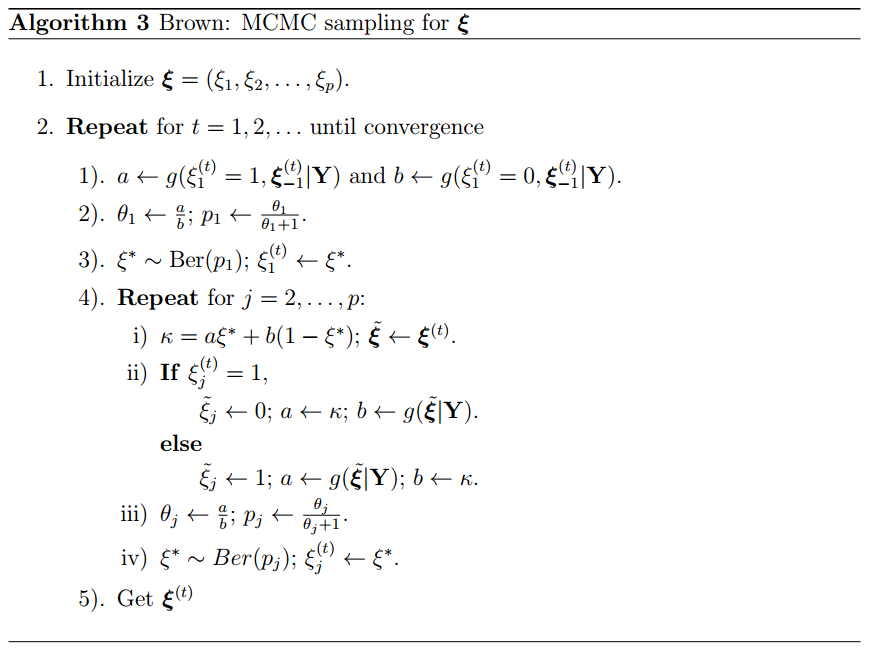
\includegraphics{alg-brown.png}

For the hyperparameter, we follow the same setting with \citep{Brown}, which are \(\delta = 2+q, \omega = 20/p, k = 2\) and \(c = 10\). Note that since our definition of inverse-wishart distribution is different from that of \citep{Brown}, the values of \(q\) and \(k\) we set here are after adjustment to make them consistent with \citep{Brown}.

\bibliography{book.bib}


\end{document}
